\section{Implementation}
In diesem Kapitel beschäftigen wir uns mit der Implementation und mit dem Aufbau von Grafana, sodass wir \gls{Cyberangriff} nach dem \gls{mitre} Matrix erkennen können. Wir gestalten unser Arbeitslabor mit \gls{container} und \glsfirst{vm}, wie in dem folgenden Diagramm:

\begin{figure}[H]
   \centering
   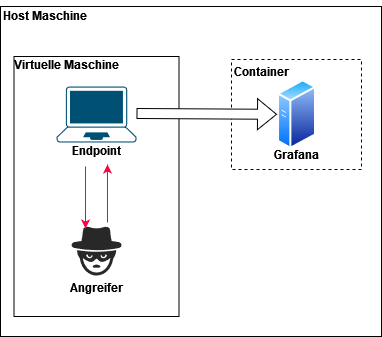
\includegraphics[width=0.8\textwidth]{assets/Arbeitslabor.drawio.png}
   \caption{Aufbau unseres Arbeitslabors \\Quelle: Eigene Quelle}
   \centering
\end{figure}

Von unserem Aufbau zielen wir, die Aufnahmen und Anpassung der Logdateien für Grafana, die Musterkerennung für die ausgewählten \glsplural{Cyberangriff} und schließlich die Warnmeldung für die Endnutzer, sodass sie sich für entsprechende Sicherheitsmßnahmen entscheiden können. Dieser Ablauf ist in dem folgenden Diagramm dargestellt:

\begin{figure}[H]
   \centering
   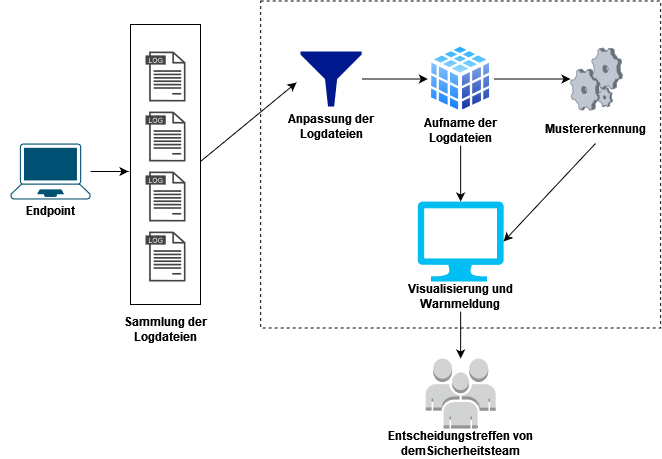
\includegraphics[width=1\textwidth]{assets/Ablauf_grafana.drawio.png}
   \caption{Erwarteter Ablauf von der Datensammlung bis zur Warnmeldung von \glsplural{Cyberangriff} \\Quelle: Eigene Quelle}
   \centering
\end{figure}

\subsection{Angriffserkennung anhand der Mitre ATT\&CK Matrix\textregistered}
Es gibt verschiedene Methode und Framework zur Vermeidung, Erkennung, und Unterbrechung von \glsplural{Cyberangriff}. \glsfirst{owasp}, \glsfirst{CKC} und \gls{mitre} Matrix sind einige Bespiele von denen, die \gls{SOC}-Teams verwenden, um Sicherheit von Systemen und/oder Netzwerken zu gewährleisten. Da die Richtlinien und Fokus von diesen Frameworks sich unterscheiden können und deswegen anderen Aufbau von unserer Struktur verlangen wurden, entschieden wir uns für die Anwendung von der \gls{mitre} Matrix für die Erkennung der \glsplural{Cyberangriff} besonders, weil dieser Framework auch an Splunk integriert ist.

\newpage
Die \gls{mitre} Matrix hat folgende Hauptnutzung \citep{Mitre_Started}:

\begin{itemize}[noitemsep]
   \item Erkennung und Analyse von Angriffstechnik
   \item	strukturierte Datensammlung über Bedrohungen
   \item	Emulieren von \glsplural{Cyberangriff} für die Anwendung an Angriffsübungen
   \item	Systemhärtung und Verbesserung der Verteidigungsmaßnahmen
\end{itemize}

Die Matrix bietet eine umfangreiche Verwendung für Unternehmen und für \gls{SOC}-Team an, um ihre wertvollen Ressource schützen und ihre Fachkenntnisse über \gls{Cybersicherheit} zu erweitern \citep{Hazel_howtousemitre}. Hier konzentrieren wir uns auf die Entwicklung und auf die Implementierung einer Methode für die automatische Erkennung und Analyse von Angriffstechnique in Grafana.

Die \gls{mitre} Framework besteht aus 14 Taktik. Zu jedem Taktik gehören Technique, die ihrerseits in Subtechniques aufgeteilt sind. Jede Subtechnique wird mit Beispielen, Härtungsmaßnahmen und Erkennungsregeln dargestellt. Die nächste Abbildung zeigt, wie diese Struktur aufgebaut ist: 

\begin{figure}[H]
   \centering
   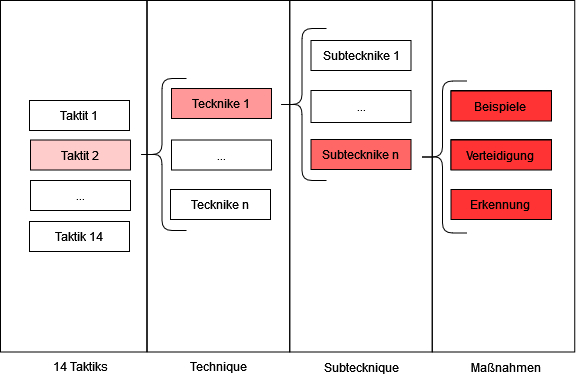
\includegraphics[width=0.8\textwidth]{assets/Mitre_structure.drawio.png}
   \caption{Struktur der Mitre Matrix \\Quelle: Eigene Quelle und \citep{Mitre_Started}}
   \centering
\end{figure}

\newpage
Die 14 Tactics sind folgende:
\begin{itemize}[noitemsep]
   \item Informationssammlung für zukünftige Angriffe 
   \item	Entwicklung von Ressource von Angreifer
   \item Erster Zugang zum Opfersysteme 
   \item Ausführung von bösartigen Coden
   \item Beharrlichkeit von System
   \item	Privilegienausweitung
   \item Vermeidung von Verteidigungssysteme
   \item Zugang zu Anmeldedaten
   \item Umgebungserkennung
   \item Seitliche Bewegung zu anderem Systemen innerhalb des Angriffsziels
   \item interne Informationssammlung
   \item Steuerung und Kontrolle (C2 - Command and Control im Original)
   \item Datenextrahierung 
   \item	Auswirkung auf die Integrität
\end{itemize}


\subsection{Auswahl des Angriffes}
In dieser Arbeit beschäftigen wir uns mit dem Tactic \quotes{Zugang zu Anmeldedaten} und deren Technique \gls{bruteforce}. Diese Technique ist in vier Subtechnique aufteilt:

\begin{itemize}[noitemsep]
   \item Erraten von Anmeldedaten 
   \item	Entschlüsselung von \glsplural{hash}
   \item \textit{\gls{stuffing}}
   \item \textit{\gls{spraying}}

\end{itemize}

Da unser Ziel hier ist Grafana, zu benutzen, um Angriffe zu erkennen, entschieden wir uns für einen einfachen reproduzierbaren Angriff, die weniger Ressource verlangt. In diesem Fall, lässt sich \gls{bruteforce} einwandfrei mit zwei \glsplural{vm} darstellen. Für diesen Angriff benutzen wir die Subtechnique \quotes{Erraten von Anmeldedaten und \textit{\gls{stuffing}}}, da sie ähnliche Erkennungmethode haben. Hier schließen wir auch die anderen Maßnahmen aus.

Die nächste Abbildung zeigt den Umfang unseres Implementationsversuchs:

\begin{figure}[H]
   \centering
   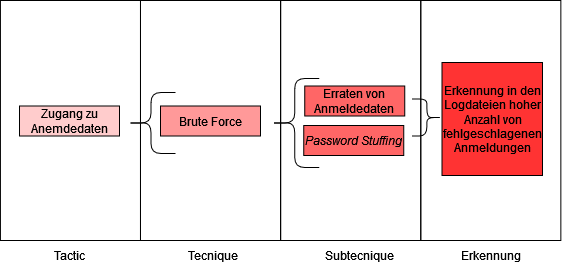
\includegraphics[width=0.8\textwidth]{assets/T1110.drawio.png}
   \caption{Analysestruktur für diese Arbeit \glsplural{Cyberangriff} \\Quelle: Eigene Quelle und \citep{Mitre_t1110}}
   \centering
\end{figure}

\subsection{Installation und Erstellung von Logdateien}

In diesem Abschnitt fokussieren wir uns folgenden Punkten:

\begin{enumerate}[noitemsep]
   \item Installation von Grafana mit \gls{container}
   \item	Installation von zwei \glsplural{vm}, eine für das Opfersystem und eine für den Angreifer
   \item	Angrifsssimulation für die für die Generierung von Logdateien
   \item Hochladen der Logdateien in Grafana
\end{enumerate}

Die Installation und Anwendung können entweder mit dem \gls{GUI} oder mit der Kommandozeilen durchgeführt werden. In dieser Arbeit benutzen wir die Kommandozeile. 

\begin{itemize}[noitemsep]
   \item \textbf{[1] Installation von Grafana mit \gls{container}}
\end{itemize}

Grafana lässt sich mit einem einzelnen Kommando installieren und in Docker \gls{container} ausführen:

\begin{verbatim}
   docker run -d --name=grafana -p 3000:3000 grafana/grafana
\end{verbatim}

Für spezifische Versionen oder andere weitere Einstellungen bietet die Dokumentation  umfangreiche Möglichkeiten an \citep{Grafana_run}. Nach der Ausführung des Kommandos ist die Anwendung schon benutzbar, wie in dem folgenden Screenshot:

\begin{figure}[H]
   \centering
   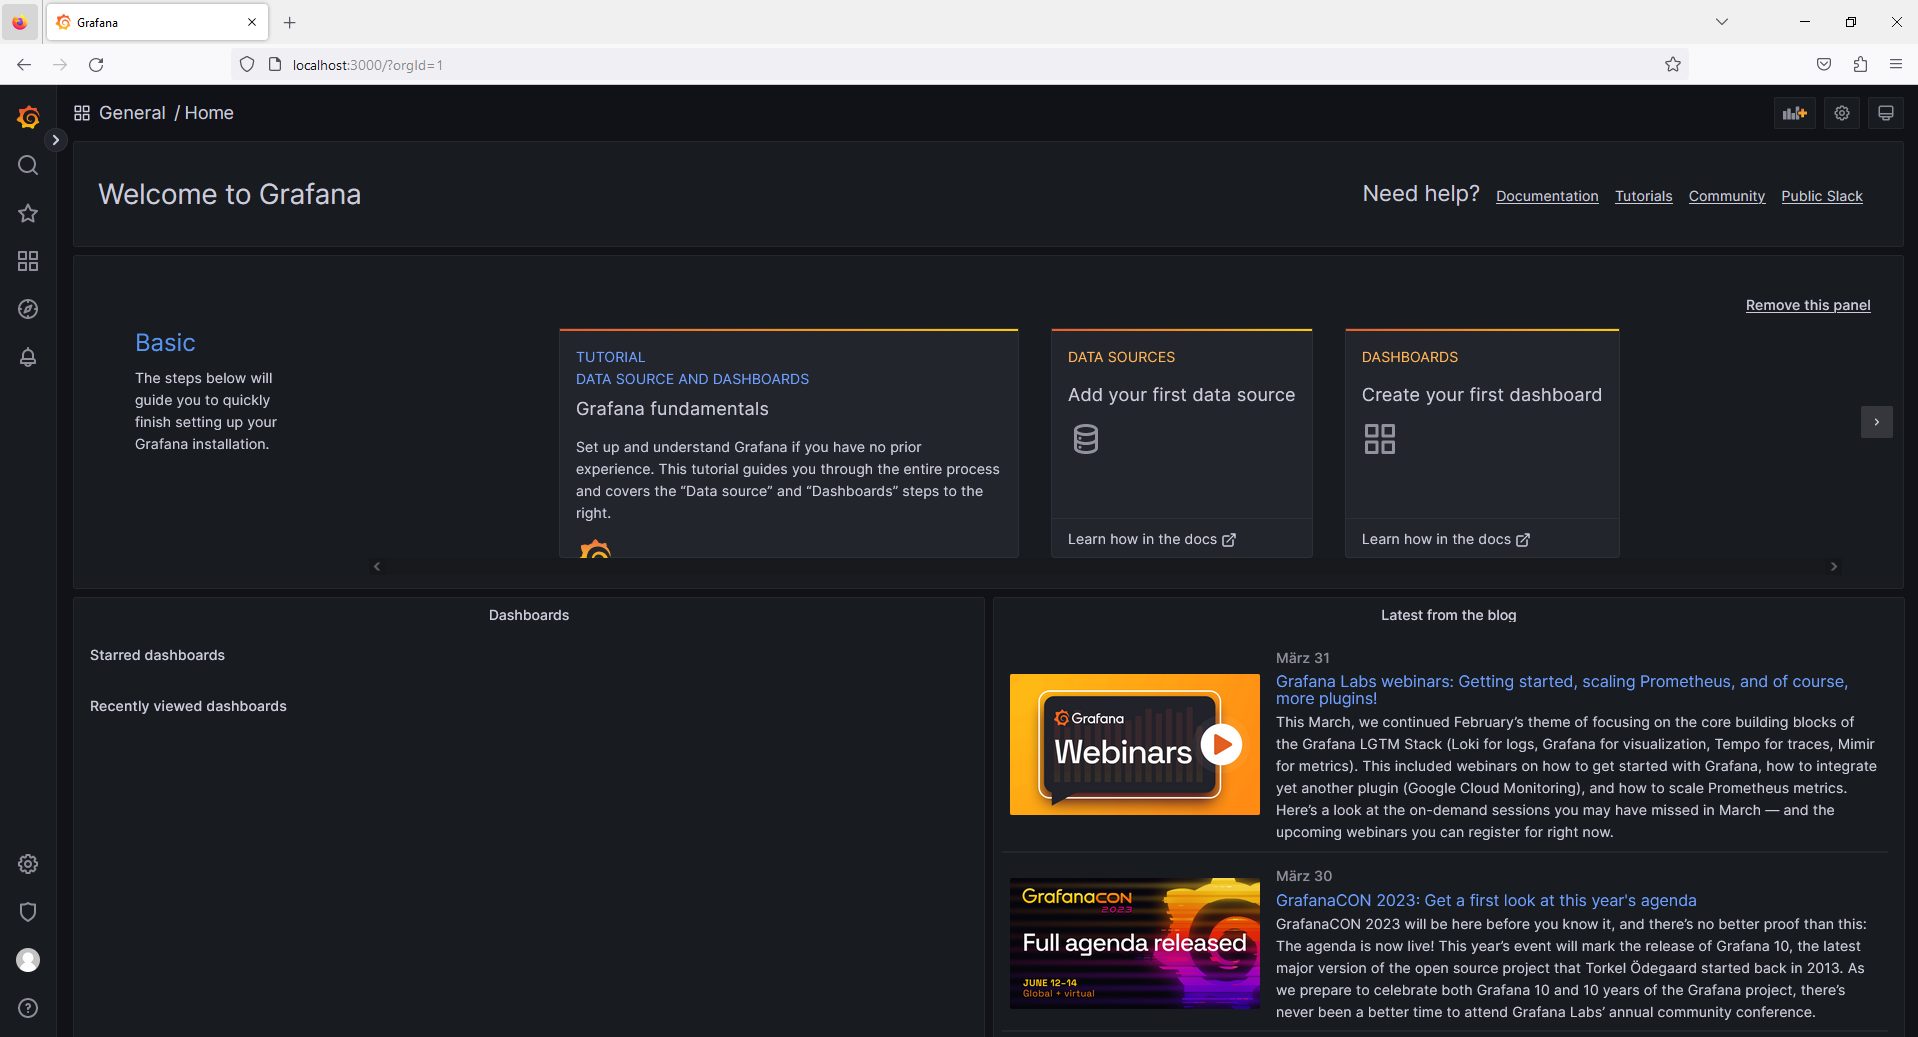
\includegraphics[width=0.8\textwidth]{assets/Installation_Grafana.png}
   \caption{Screenshot der Willkommensseite von Grafana\\Quelle: Eigene Quelle und \citep{Grafana_Logs}}
   \centering
\end{figure}

\begin{itemize}[noitemsep]
   \item	\textbf{[2] Installation von zwei \glsplural{vm}, eine für das Opfersystem und eine für den Angreifer}
\end{itemize}

Die beiden \glsplural{vm} sind \quotes{\gls{kali} vorgebaute \glsfirst{vm}} und \quotes{\gls{ubuntu} Server 22.04.2} in ihren standardmäßigen Einstellungen. Beiden Maschinen lassen sich aus der jeweiligen Schritte Dokumentation einwandfrei installieren \citep{kali_vm} und \citep{Ubuntu_server}. Für das Opfersystem entschieden wir uns für eins des zehn meisten verwendeten Passwort in Deutschland laut einer Umfrage \citep{silicon_passwort}: qwertz.  

\begin{itemize}[noitemsep]
   \item	\textbf{[3] Angrifsssimulation für die für die Generierung von Logdateien}
\end{itemize}

Für den Angriff verwenden wir folgenden Tools:

\begin{itemize}[noitemsep]
   \item	\glsfirst{ssh}
   \item \gls{hydra}
\end{itemize}

In diesem Szenario schickt \gls{hydra} gleichzeitig mehrere Authentifizierungsversuche zum Opfersystem. Das Tool verwendet ein sogenanntes  Wörterbuch mit verschiedenen Einträgen, die als Passwörter dienen. Für unseren Test benutzen wir die bekannten Datei \gls{rockyou}. Die folgenden Diagrammen stellen unsere beiden Angriffe dar:


\begin{figure}[H]
   \centering
   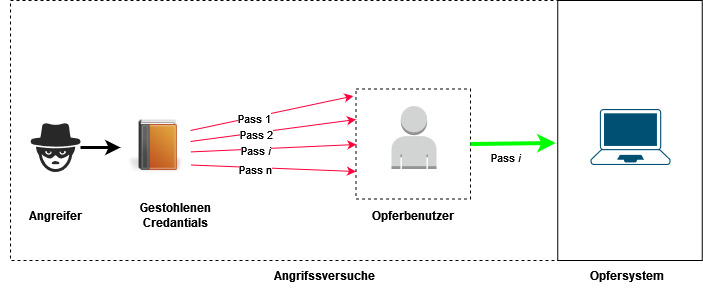
\includegraphics[width=0.8\textwidth]{assets/Stuffing.jpg}
   \caption{\textit{\gls{stuffing}}\\Quelle: Eigene Quelle und \citep{Nguyen_stuffing}}
   \centering
\end{figure}


\begin{figure}[H]
   \centering
   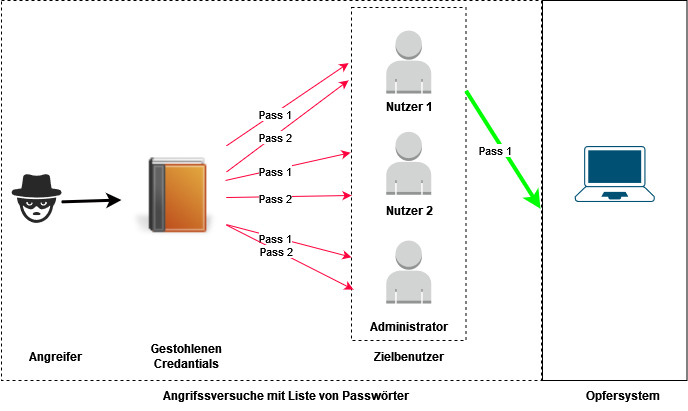
\includegraphics[width=0.8\textwidth]{assets/Spraying.jpg}
   \caption{\textit{\gls{spraying}}\\Quelle: Eigene Quelle und \citep{Swathi_spraxy}}
   \centering
\end{figure}


\subsection{Aufbau der Erkennungsregel für den ausgewählten Angriff}
Der \gls{bruteforce} lässt sich durch die Anzahl des fehlgeschlagen Anmeldungsversuchs erkennen \citep{Selvaganesh_SplunkBruteForce}. Wir bearbeiten eine Situation, in der es keine Gegenmaßnahmen, wie Kontosperre nach \textit{n} beliebigen Versuchen oder \gls{mfa}, implementiert sind. Das folgende Aktivitätsdiagramm stellt einen allgemeinen Ablauf eines Anmeldungsverfahrens dar:

\begin{figure}[H]
   \centering
   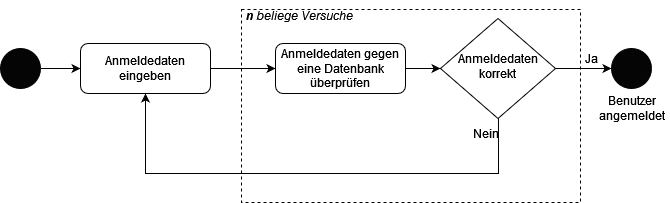
\includegraphics[width=0.8\textwidth]{assets/Anmeldeverfahren.drawio.png}
   \caption{Allgemeiner Ablauf eines Anmeldungsverfahrens \\Quelle: Eigene Quelle und \citep{Selvaganesh_SplunkBruteForce}}
   \centering
\end{figure}

\textcolor{red}{\textbf{Regel von SPLUNK hinzufügen, wie sollten unsere Regel aussehen}}

\textcolor{red}{\textbf{statische vs dinymische Regel}}





\subsection{Bewertung der Daten in Grafana}
Hinzufügen der Logdateien und Erstellung von Regeln zur Erkennung des Angriffes
Diagramm der Nutzung von Grafana

\subsection{Normalisierung der Logdateien mit Zeek}
Diagramm der Nutzung von Grafana und Zeek

Hier werden die Schritte für die Installation und Sammeln von Daten beschrieben.

- Implementation in Container %https://rdr-it.com/elk-installation-configuration-un-siem-docker/


\subsection{Sammlung von Server-Log Dateien}

\subsection{Normalisierung der Log-Dateien}





